\section{Introduction}
\subsection{Motivation}
With the rise of simulation and big data analytics as new foundations of all modern science,
access to large scale \ac{HPC} systems has become paramount for good research. Furthermore,
as the area of machine and deep learning progresses, with models containing over one billion
parameters \cite{gpt4param},  local computation becomes everless feasable, resulting in the 
rise of \ac{HPC} usage amongst various domains.\\

This report is written as an addition to my student research at the \ac{GWDG}. The \ac{GWDG} is the
data center of the University of Göttingen and the data and IT competence center of the 
Max Planck Society with its own \ac{HPC} department, running four large scale \ac{HPC} systems:
The \ac{SCC}, Emmy, Grete, and CARO:
\begin{itemize}
\item \textbf{\ac{SCC}}\cite{SCC}: The \ac{SCC} is the oldest cluster maintained 
by the \ac{GWDG}. Its user group is comprised of all researchers of the Max Planck Society as 
well as all (student) researchers of the University of Göttingen. It is a very heterogenous system,
based on several different CPUs and GPUs generations, located over several locations within 
Göttingen. In total, it has 18,376 CPU Cores, 99 TB RAM and 5.2 PiB of Storage.
\item \textbf{Emmy}\cite{Emmy}: Together with the Lise\footnote{
\url{https://www.zib.de/research_services/supercomputing}} cluster provided by the ZIB, Emmy is 
part of  the fourth supercomputer generation of the HLRN\footnote{Norddeutscher Verbund für Hoch- 
und Höchstleistungsrechnen \url{https://www.hlrn.de/}}. It can be used by all HLRN and NHR users.
Ranking 133th at the TOP500\footnote{As of November 2023.}, Emmy is the biggest cluster hosted by
the \ac{GWDG}. It consists of 111,464 CPU Cores distributed over 1423 compute nodes resulting 
in a total peak compute power of 5.95 PetaFLOP/s.
\item \textbf{Grete}: Grete is a GPU \ac{HPC} cluster, formally part of the NHR system.
It features 158 nodes with 2 AMD Epyc 7513 CPUs and four NVIDIA A100 GPUs each, connected through fast
Infiniband fabric. As of November 2023, Grete is rank 142 of the TOP500.
\item \textbf{CARO}\cite{CARO}: Analagously to Emmy provided for the NHR, CARO is a compute cluster
hosted for the DLR\footnote{Deutsches Zentrum für Luft- und Raumfahrt \url{https://www.dlr.de/en}}.
With its 1364 compute nodes with 175,744 CPU Cores and 3.46 PetaFLOP/s it ranks 228th on TOP500.
\end{itemize}

As the sheer number of nodes makes individually inspecting each one impossible, a centralized
monitoring solution is required. Beyond getting an basic understanding on which node is alive, 
monitoring systems serve several important purposes. With an aggregated view, system admins can
understand the usage patterns. Furthermore, it can be used as a means of load balancing 
for detecting preventable bottlenecks such as suboptimal job queue usage. Additionally, monitoring
allows for better demand analysis and forecasting, allowing for more efficient, just in time 
hardware upgrades.

\subsection{Goals and Contributions}

As the time of this writing, the GWDG has two different, Grafana-based monitoring solutions for 
the \ac{SCC} and Emmy/Grete. The goal of this report is to evaluate the performance viability of
unifying both monitoring solutions, replacing \ac{SCC}'s InfluxDB\footnote{
\url{https://www.influxdata.com/products/influxdb-overview/}} and Telegraf\footnote{
\url{https://www.influxdata.com/time-series-platform/telegraf/}} with Prometheus and 
\texttt{node\_exporter}.
As part of this, the following contributions were made:
\begin{itemize}
\item Designing a methodology for benchmarking a pull-based monitoring system.
\item Designing a methodology for benchmarking a pull-based monitoring client daemon, both in 
terms of throughput and the performance degradation caused to typical, throughput-oriented 
\ac{HPC} load.
\item Benchmarking the performance and scalability of Prometheus for a \ac{HPC} use case.
\item Benchmarking the performance and performance penalty of \texttt{node\_exporter} for a 
\ac{HPC} use case.
\end{itemize}

\subsubsection{Structure}
Starting with Section 2, the general topics of monitoring, time series databases and
Prometheus get introduced. Related work about time series database performance will be analyzed.
After that, in Section 3, the benchmark methodology for both Prometheus itself as well as
\texttt{node\_exporter} will be explained. Then, in Section 4, the results of those benchmarks
will be shown. After a short discussion in Section 5, the work will be concluded in Section 6.

\section{Background: Monitoring}
Monitoring consists of 2 important components. On the one hand, it is the continuous 
collection of mostly numerical data and metrics from various systems. On the other hand, it 
is the aggregation and analysis of this collected data/metrics within a certain period of 
time, up to real-time monitoring.

Several different kinds of metrics can be analyzed using monitoring systems. From typical
system metrics such as CPU, RAM, disk, or network usage to monitoring whole server racks
with power and cooling statistics as well as application specific metrics such as databases
or webservers.

Most monitoring systems follow the collector/database/dashboard architecture. On each node,
a \emph{collector} is running as a daemon, exposing the internal metrics for an centralized
database, aggregating all nodes. Those databases are usually either general, document-based
NoSQL databases such as MongoDB\footnote{\url{https://www.mongodb.com/}} and 
Elasticsearch\footnote{\url{https://www.elastic.co/elasticsearch}} or specialized \acp{TSDB}
such as InfluxDB\footnote{\url{https://www.influxdata.com/}} or Prometheus\footnote{
\url{https://prometheus.io/}}.

To provide an taxonomy, most monitoring systems can be categorized on two dimensions:

\paragraph{Cloud-based or On-Premise:} Monitoring systems can either be managed, cloud-based 
or self-hosted, on-premise services. Both have their advantages and disadvantages.

Cloud-based monitoring services such as Datadog\footnote{\url{https://www.datadoghq.com/}}
or Splunk\footnote{\url{https://www.splunk.com/}} have several advantages. By using an 
externally hosted service, it simplifies the overall monitoring maintenance. By not requiring
hardware for another service, it lowers the barrier of entry. Furthermore, since the whole
monitoring stack is written by the same manufacturer, it allows for tighter integration.

On-Premise hostings, on the other hand, also have several advantages over the cloud-based 
solutions. Since they are part of the local network, they are easier to integrate into current
infrastructure, even those parts that one doesn't want to publically expose such as Active 
Directory or other Identity Management Solutions. Additionally, it mitigates potential security and privacy risks, especially for data
that could either pose a security risk such as showing applicable vulnerabilities or data that is
legally not allowed to be processed off-premise such as sentitive user data. Lastly, while the 
software stack is more heterogenous, it allows for more specialization based on the users needs.

\paragraph{Push or Pull:} There are two different paragigms in data gathering:

In the more common \emph{push} paradigm, the data-collecting daemon sends the data to an API 
endpoint. This has multiple advantages: First, it is easier for firewalls, because it does not
need any inbound connection establishment. It is also less overhead for the \ac{TSDB} since it
just needs to passively recieve the data. Lastly, it is easier to send non-aggregated raw data,
since the client can decide when it has enough data to send to the database.

In the \emph{pull} paradigm, the \ac{TSDB} itself iterates over, and fetches all metrics, which
are exposed as newline-seperated key-value pairs through an specified HTTP-endpoint. The biggest
advantage is that the \ac{TSDB} can't be overwhelmed with requests since it implicitly rate-limits
itself through the amounts of outgoing requests. Furthermore, it allows for lazy and just-in-time 
fetching of data, reducing the overall overhead in the network.

The \ac{GWDG} uses both push and pull \acp{TSDB} in the \ac{SCC} and Emmy cluster respectively. 

\subsection{Current Architecture: GWDG SCC}

The \ac{SCC} uses an push-based architecture: On every node, the plugin-powered Telegraf 
daemon collects all metrics, which are then send to the InfluxDB \ac{TSDB}. Finally, this database
gets queried using the legacy InfluxQL by Grafana\footnote{\url{https://grafana.com/}} as 
configured in the dashboards.

\begin{figure}[H]
  \centering
  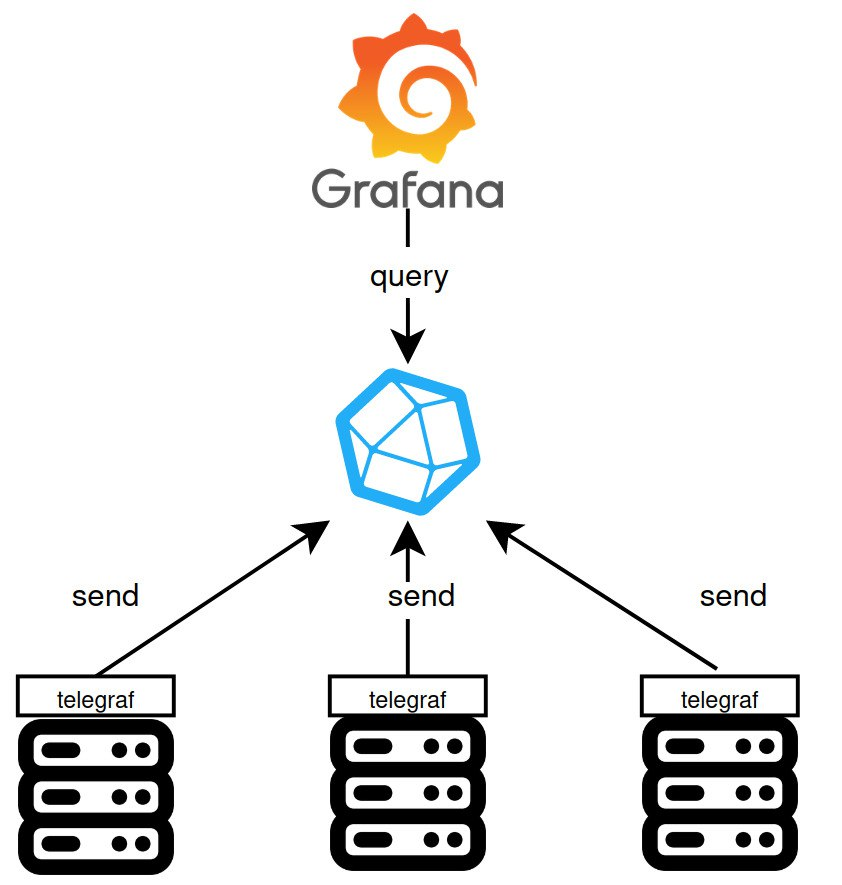
\includegraphics[width=0.5\textwidth]{./assets/influx.jpeg}
  \caption{The InfluxDB-based push-setup for the SCC.}
\end{figure}


\subsection{Current Architrecture: HLRN Emmy}
For Emmy, a pull-based architecture is used. The node\_exporter\footnote{
\url{https://github.com/prometheus/node_exporter}} exposes the \texttt{/metrics} HTTP endpoint, to which
the Prometheus database connects to when fetching the data. The aggregated data also gets queried
through pre-made Grafana dashboards with PromQL.

\begin{figure}[H]
  \centering
  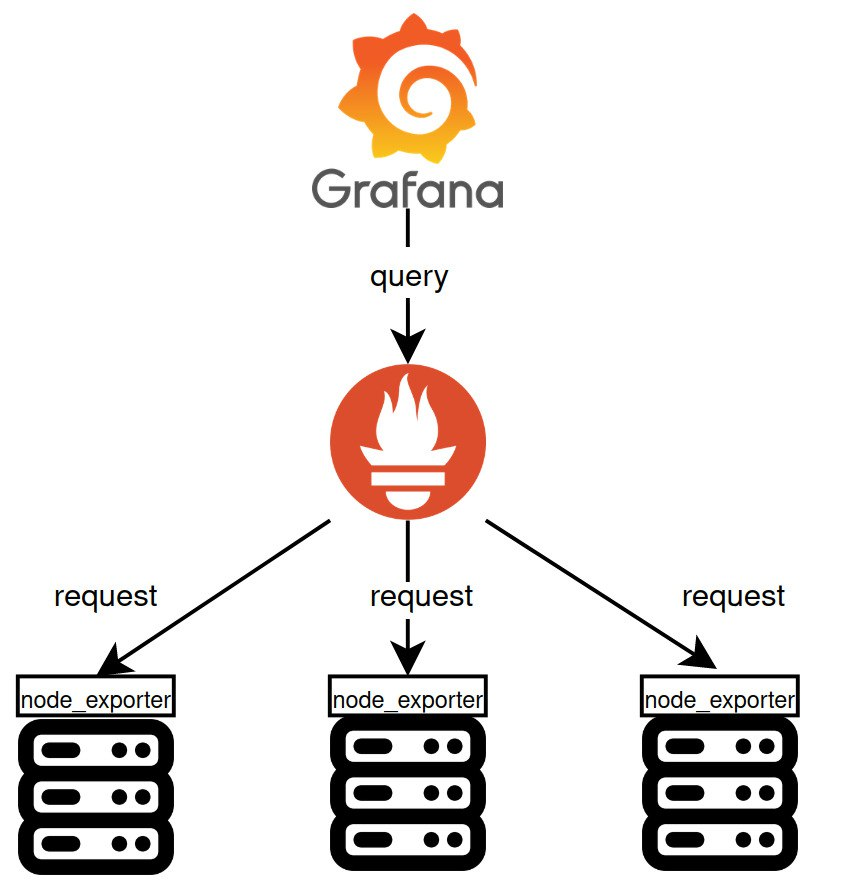
\includegraphics[width=0.5\textwidth]{./assets/prometheus.jpeg}
  \caption{The Prometheus-based pull-setup for Emmy.}
\end{figure}

\subsection{Prometheus}
More than just a \ac{TSDB}, Prometheus is a pull-based systems monitoring toolkit. Originally 
developed at SoundCloud, it is now a non-commercial open source project hosted by the \ac{CNCF},
which is a part of the Linux Foundation. The clients expose the pull metrics via \texttt{node\_exporter} or other custom tooling,
that then get scraped by the Prometheus server into its \ac{TSDB}, which can then be queried through
PromQL, its own query language.

\begin{figure}[H]
  \centering
  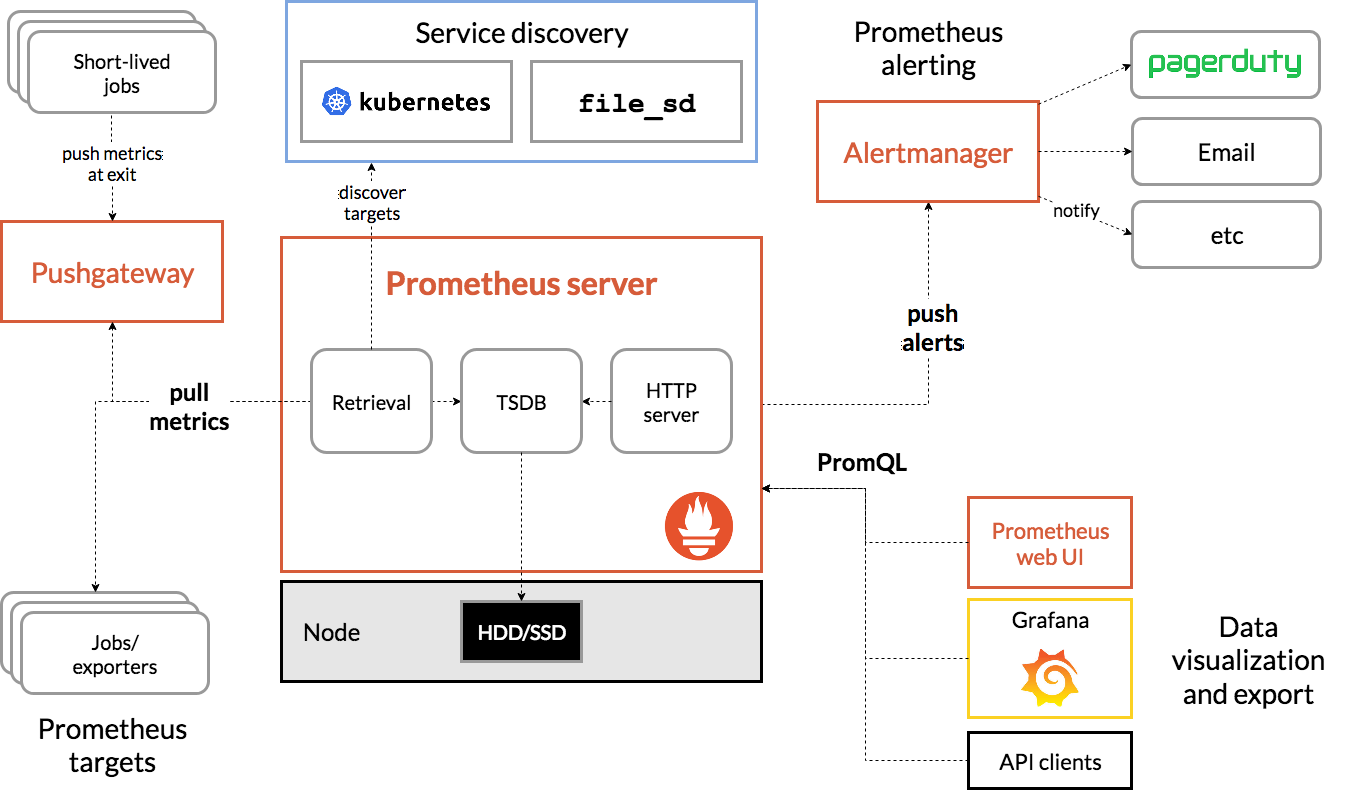
\includegraphics[width=\textwidth]{./assets/promarch.png}
  \caption{Prometheus high level architecture \cite{promarch}.}
\end{figure}

\subsection{TSDB Performance Evaluation}
While there are several papers on \ac{TSDB} performance evaluation, most benchmarking was mainly
done by different vendors. In this section, we will cover one publication as well as two
industry standards for push and pull based database benchmarking respectively.

The most actively maintained academic benchmark was first published by Liu and Yuan in 2019 \cite{benchmark_paper}.
It is maintained to this day. While it surrently only supports Push-based metrics, it supports not
only traditional \ac{TSDB} such as InfluxDB or TimeScaleDB but also classical SQL-based databases
such as SQLite or Microsoft SQL Server. It also supports several benchmarking scenarios testing
both write and query performance.

But the canonical benchmarking suite for push-based \acp{TSDB} is the \ac{TSBS} \cite{tsbs}, 
maintained by Timescale, the maintainer of timescaledb\footnote{\url{https://www.timescale.com/}}, a 
time-series database packaged as an PostgresSQL. Initially developed by an external contractor
for InfluxData as \texttt{influxdb-comparisons} \cite{influxcomp}, it supports most \acp{TSDB}.
It is split into 3 different, purely distinct phases: Data and query generation, data insertion,
and query execution. This is done to minimize the load generator overhead for more reliable results.

Due to the constant load configured on the server side instead of the load generator side, pull-based
\ac{TSDB} benchmarking is more difficult. Although still pretty new, the only well maintained
benchmark suite for prometheus-like systems is \texttt{prometheus-benchmark} \cite{prombench}, developed by 
VictoriaMetrics\footnote{\url{https://victoriametrics.com/}}, a competitor to Prometheus. It supports
VictoriaMetrics as well as Prometheus based Grafana's Mimir\footnote{\url{https://grafana.com/oss/mimir/}}
and the \ac{CNCF}-maintained Prometheus clustering solutions Cortex\footnote{\url{https://github.com/cortexproject/cortex}}
and Thanos\footnote{\url{https://github.com/thanos-io/thanos/}}. Unfortunately, it can not be used for
this benchmark as it expects a Kubernetes-based cloud environment while this use case is around \ac{HPC} usage.

Unfortunately, due to the competitive nature of the highly funded No-SQL startup space, both
benchmarks suits are susceptible to commercial incentives.


\section{Benchmark Methodology}
This section will cover the design and methodology behind all benchmarks. In particular, the following
benchmarks were designed as part of this report:

\begin{itemize}
  \item Measuring the isolated performance of the metric gathering function within the \texttt{node\_exporter} daemon.
  \item Measuring the end-to-end performance and stress test resilience of the \texttt{node\_exporter} daemon with different HTTP load generators.
  \item Measuring the scalability of Prometheus by increasing the number of daemons to fetch from.
  \item Measuring the performance penalty of \texttt{node\_exporter} on an running \ac{HPC} job (jitter-benchmark).
\end{itemize}

Note that the code for all benchmarks \cite{my_repo} as well as the patched \texttt{node\_exporter} \cite{my_node_exporter}
can be found on Github.

\subsection{Setup}

For the \texttt{node\_exporter} performance benchmarks as well as the Prometheus benchmark, an \ac{HPC} 
gcn2 type node from the HLRN Emmy cluster was used. This node has two Xeon Platinum 9242 with 48 cores each
as well as 376GB of RAM. The servers were solely used for the benchmarks, thus resulting in
no noisy neighbour problems.

In order to facilitate a more minimal operating system with less running services, the jitter-based 
performance penalty benchmark was done locally on a Thinkpad T14 Gen 1 running a minimal
Ubuntu Server 22.04 LTS with all non-essential services killed. The Thinkpad has a quad-core Intel i5-10210U and 16GB of RAM.

The \texttt{node\_exporter} benchmarks uses a precompiled node exporter of version 1.7.0\footnote{With the following collectors enabled: cpu, cpufreq, infiniband, meminfo, netdev, vmstat.}
For the isolated metric gathering benchmark, 
\texttt{node\_exporter} was forked from version 1.7.0. For Prometheus, a Ubuntu 22.04 based singularity
container was used as a basis, containing a Prometheus version 2.45.1. The Dockerfile is also available
in the repository \cite{my_repo}.

\subsection{\texttt{node\_exporter}}
\subsubsection{Metric Gathering}

When requesting all metrics via the \texttt{/metrics} HTTP endpoint, \texttt{node\_exporter} runs the following
function:

\begin{listing}[H]
  \inputminted{go}{./gather.go}
  \caption{How the metrics are collected in \texttt{collector/collector.go}}
\end{listing}

So when requesting the metrics, \texttt{node\_exporter} spawns a new green thread for each metric plugin, 
awaiting all results in a fork-join like model with a semaphore. Instead of benchmarking the single function
by mocking a realistic application state, the Collect function was patched as follows:

\begin{listing}[H]
  \inputminted{go}{./gather_patched.go}
  \caption{The patched collector measuring the collection time. Note that the \texttt{RealCollect} function contains the same code as the unpatched \texttt{Collect}.}
\end{listing}

Further small patches had to be done to fix any errors, see the reporitory for more information \cite{my_node_exporter}.

\subsubsection{End to End}
The end-to-end benchmarks measured the throughput of the client exposing the metrics using traditional HTTP benchmarking. In particular, two different
benchmarking tools were used:
\begin{itemize}
  \item \textbf{wrk} \cite{wrk} is a popular, CLI-based HTTP benchmarking tool written in C. Due to its optimized
    performance it can serve as a baseline optimal throughput. In order to further improve throughput, it keeps
    all HTTP connections open between requests.
  \item \textbf{go-wrk} \cite{go-wrk} is a reimplementation of wrk in the Go programming language, using gos
    green threads and standard \texttt{net} library for the load generation.
\end{itemize}
All benchmarks are continuously measured using \texttt{vmwstat 1}. The benchmarks can be divided into three different kinds.
\begin{enumerate}
  \item \textbf{wrk sequential}: Using a single thread and a single connection, this is the most realistic load,
    as metrics are usually only crawled by a single Prometheus server as well. This is also the simplest possible benchmark;
    just send as fast as possible.
  \item \textbf{wrk parallel}: Scaling along the number of open HTTP connections and threads. This is for creating the maximally possible throughput, although it is not realistic since prometheus does not open multiple HTTP connections to the same \texttt{node\_exporter}.
  \item \textbf{go-wrk parallel}: Scaling along the number of go routines/green threads. This is a more realistic load, as it most behaves like Prometheus. Both Prometheus and go-wrk use the same underlying request library, both do not keep HTTP connections open between requests and both use go routines for parallelism.
\end{enumerate}
The benchmarks work as follows: In an outer loop, we scale around the number of processes consumed by the \texttt{node\_exporter} by changing the \texttt{GOMAXPROCS} environment variable of the underlying go runtime. Note that even with single threading go routines can still highly improve performance by hiding I/O idle times between different metrics fetching. For each parallelism, we scale the software as described above, sending against the \texttt{/metrics} endpoint, which in turn starts node exporter to refetch and return the newest values. By measuring how often this request can be done and the latency it took, the performance can be evaluated.

Note that this complete benchmarking pipeline is scripted out and automated into a single SLURM job.
\subsubsection{Jitter}
While the performance of the metric collector itself is important, it can reasonably be assumed that they are able to run well on big \ac{HPC} machines. From a raw compute providers standpoint, the more interesting question is whether the metric collection overhead is managable, i.e. the performance degradion of the running jobs are significant. 

Performance degration is hard to measure. For once, \ac{HPC} systems, while running a minimal operating system, are still very complex running many different daemons. It is not sufficient to just measure the time a single threaded metric collection takes and take that share times the CPU clock speed; other performance losses such as flushed CPU caches or bad OS scheduling can incur even bigger losses than the actual runtime. As previously shown \texttt{node\_exporter} spawns a new go routine for each metric, which could result in a lot of cache invalidation.

The approach used in this report is a more realistic one. We have written an MPI-based program running the following pseudo-code:
\begin{listing}[H]
  \inputminted{C}{./jitter.c}
  \caption{A simplified C-style pseudo code of the jitter program.}
\end{listing}
This code just, as fast as possible, measures the current time on as many processes as spawned via MPI. By using barriers, it can be assured that the processes do not get out of sync, creating unexpected load spikes. Once the \texttt{node\_exporter} metrics get requested, a slowdown in measurements can be seen, which can then be analyzed in order to quantify the severity of the interference.

\subsection{Prometheus}
As examplained in the background section, benchmarking pull-based \ac{TSDB} monitoring solutions is comparitively complicated. Using normal push-based APIs, one can just use traditional HTTP load generators such as JMeter. This is not possible, since the \ac{TSDB} itself has to start each request to the metric collector daemons. So, instead of measuring how many requests the database can handle, it will instead be measured how many clients Prometheus can pull from until its pull frequency suffers. This is done my completely mocking the \texttt{node\_exporter} collection daemon and counting the number of times each node was requested by Prometheus.

More specifically, Prometheus gets an autogenerated config\footnote{Example config in Appendix.} that configures it to scrape all targets, i.e. all \texttt{node\_exporter}, to be checked every 10 seconds. This benchmark runs 10 minutes. This means that, once all clients report to be crawled significantly less than 60 times, Prometheus was not able to handle all mock clients anymore, which implies that the load was too much.

The mock clients were created using Python 3.9 with FastAPI\footnote{\url{https://fastapi.tiangolo.com/}} 0.104 and the Uvicorn\footnote{\url{https://www.uvicorn.org/}} 0.24 as an \ac{ASGI} implementation. Each node exposes 50 integer metrics, although this is configurable. Instead of just using a static website, each metric updates randomly in order to circumvent any kind of caching optimization on Prometheus side.\\

For randomness, Python uses a standard mersenne twister with a timestamp as a seed value. Since all mock APIs are spawned at approximately the same time, it could happen that multiple nodes have the same mock values. Since it was not known whether Prometheus optimizes/joins multiple nodes with the same values, this had to be fixed.

One could theoretically call \texttt{/dev/urandom} for every number, but both the OS call and the Python bytes-to-number conversion are too costly. So instead, when starting the number, the following prodecure is run to insure cryptographical uniqueness between the different mock clients:
\begin{itemize}
  \item Get 8 random bits from \texttt{os.urandom}, interpret as unsigned byte $b$.
  \item Let the mersenne twister generate $b$ random numbers as a warmup.
  \item Use the warmed up mersenne twister as a random number generator.
\end{itemize}

When terminated\footnote{This is done via explicit signal handling.}, each mock client dumps the amount of requests it recieved into a text file. Concurrent writes are fixed by letting each client create its own text with with its current process id interpolated into the filename.\\

To summarize, the high level fully automatized workflow works as follows:
\begin{itemize}
  \item The number of mock clients are provided as an CLI parameter in the form of a free port range to use.
  \item Given that port range, a Prometheus config is dynamically generated, configuring the service to scrape each port once every 10 seconds. That config is later bind-mounted into a custom Prometheus singularity container.
  \item Spawn all mock clients; sleep $2 \cdot \text{\texttt{number\_of\_clients}}$ for them to start.
  \item Record server utilization in 1 second resolution using \texttt{vmstat 1}.
  \item Start the singularity container with the config and a data directory bind-mounted in.
  \item Sleep for 10 minutes (the actual benchmark).
  \item Terminate\footnote{The exact signal is \texttt{SIGTERM}.} prometheus, then \texttt{vmstat}, then all mock exporter.
\end{itemize}

\section{Results}
This section will cover the results of the aforementioned benchmarks. First, it will go over the performance of the \texttt{node\_exporter} itself, which measures how performant the daemon is at collecting all metrics of a single node. After that, the focus will be on the overhead on normal computation load incured by the \texttt{node\_exporter}. Lastly, the results of the benchmark of Prometheus itself will be covered.

Note that all benchmark scripts as well as analysis code can be found in the accompanying GitHub repository.
\subsection{\texttt{node\_exporter} Performance}
\paragraph{Patched Node Exporter:} First, we start looking at the metric gathering benchmark, i.e. running the metric gathering 1000 times in a loop without the overhead of HTTP and the Go router. The following probability density functions were computed using \texttt{seaborn}s kernel density estimation.
\begin{figure}[H]
\centering
\begin{subfigure}{.5\textwidth}
  \centering
  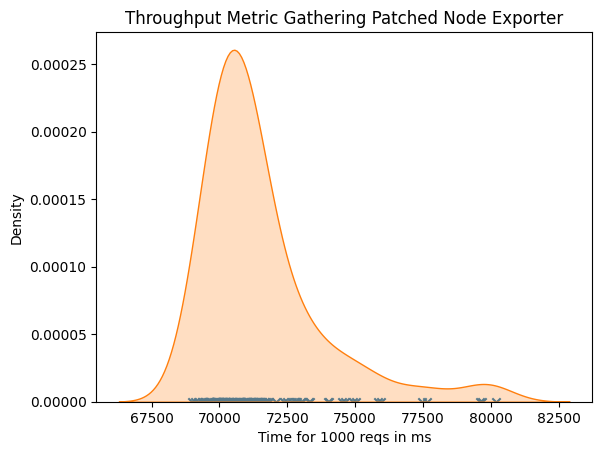
\includegraphics[width=\textwidth]{./plots/patched_node_exp_time_per_1000_reqs.png}
  \caption{}
\end{subfigure}%
\begin{subfigure}{.5\textwidth}
  \centering
  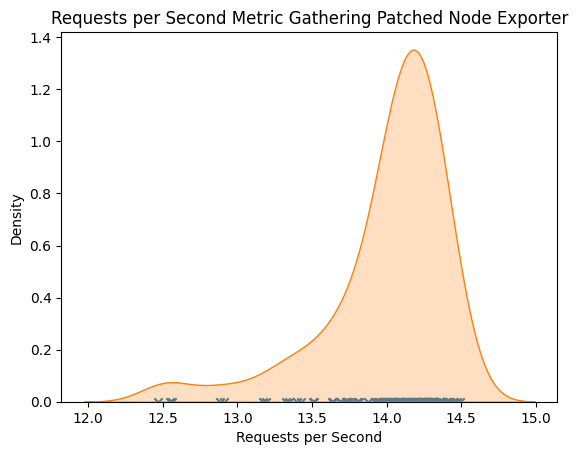
\includegraphics[width=\textwidth]{./plots/patched_node_exp_reqs_per_sec.png}
  \caption{}
\end{subfigure}
  \caption{A kernel density estimation of the results. a) showing the raw times it took to collect all metics 1000 times. b) calculated the approximated requests per second from the initial data.}
\end{figure}
Calculating from the original data, the average request took 71ms, which is an equivalent of 13.99 requests per second, which shows that there is plenty of spare time for adding additional metrics. For the realistic use case of running Prometheus as the monitoring solution of the \ac{SCC}, it can be assumed that the metrics will be fetched around once every 10 seconds. This results in 0.71\% of the time a go process will be running, allocating a single CPU. As previously mentioned, the node used has two Xeon Platinum 9242 with 48 cores, i.e. 96 threads, each. Depending on how well multithreading is utilized at that moment, this results in somewhere between 0.014\% and 0.0074\% of the total compute time. Although this data shows that the direct resource overhead incured by \texttt{node\_exporter} is negligable note that this computation does not include the performance penalty on the other jobs and thus can be seen only as a loose lower bound.\\

\paragraph{Node Exporter HTTP benchmarking:} The results of this benchmark are two-fold. First, it was analyzed how well it scales with with parallelism under moderate load. For that, a single threaded \texttt{wrk} load generator\footnote{Using multiple open HTTP connections} was used while the number of processes available to the Go runtime was increased between benchmarks:

\begin{figure}[H]
  \centering
  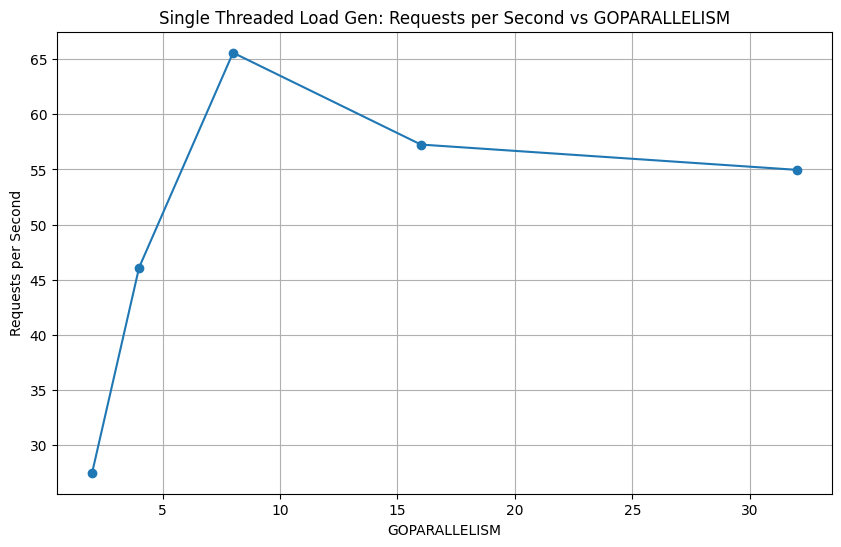
\includegraphics[width=0.7\textwidth]{./plots/node_exporter_performance_per_parallelism.png}
  \caption{The requests per second given the amount of processes available for Gos runtime. Note that $n=1$ failed while benchmarking due to an error in the benchmark pipeline.}
\end{figure}
It can be seen that beyond 8 processes the performance decreases, due to the overhead being higher than the performance gains made my the extra parallelism. Furthermore, with 2 processes, the whole end-to-end request\footnote{Excluding a realistic round trip time since the request was done against \texttt{localhost}} was completed around 27.5 times per second.\\

Lastly, it was tested how resilient the \texttt{node\_exporter} is against very heavy load. For this, the \texttt{wrk} load generator was used using 16 threads. The benchmark was scaled in two dimensions: Both in the number of concurrent HTTP connections between \texttt{wrk} and \texttt{node\_exporter} as well as the number of processes available to the Go runtime.
\begin{figure}[H]
\centering
\begin{subfigure}{.5\textwidth}
  \centering
  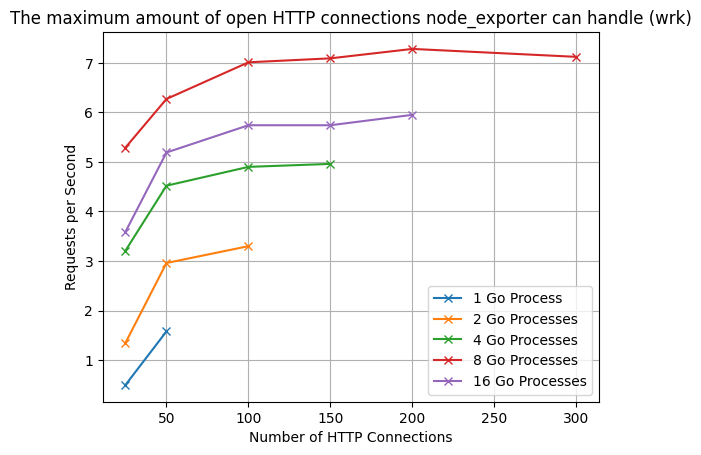
\includegraphics[width=\textwidth]{./plots/node_exporter_throughput.png}
  \caption{}
\end{subfigure}%
\begin{subfigure}{.5\textwidth}
  \centering
  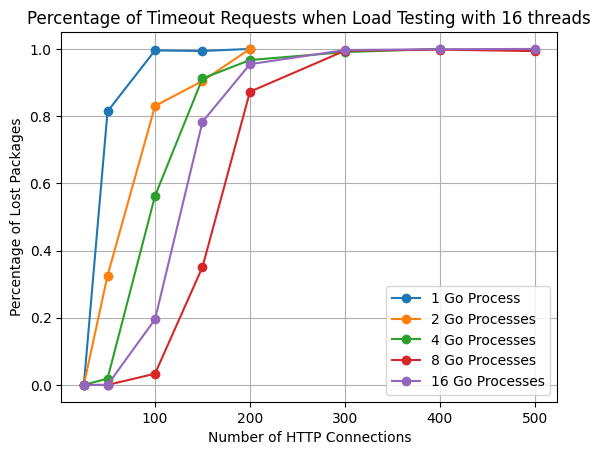
\includegraphics[width=\textwidth]{./plots/node_exporter_errors.png}
  \caption{}
\end{subfigure}
  \caption{a) shows the average throughput and b) the percentage of requests which timed out.}
\end{figure}
This benchmark shows that \texttt{node\_exporter} performs very poorly under heavy load. Even with the previously found optimum of 8 OS processes, it results in over 80\% of requests timed out when sending under a heavy load.
\subsection{\texttt{node\_exporter} Performance Penalty (Jitter)}
The following histograms are measurements from the jitter benchmark ran on an 8 thread CPU, resulting in $n=134,217,728$ data points per plot.
% jitter:
\begin{figure}[H]
\centering
\begin{subfigure}{.42\textwidth}
  \centering
  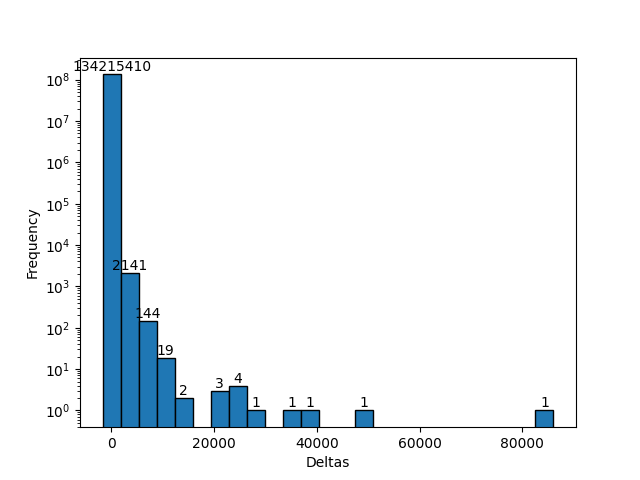
\includegraphics[width=\textwidth]{./plots_jitter/jitter/output_size_1_rank_0_25.png}
  \caption{jitter single thread\\$t=2.437996071$}
\end{subfigure}%
\begin{subfigure}{.42\textwidth}
  \centering
  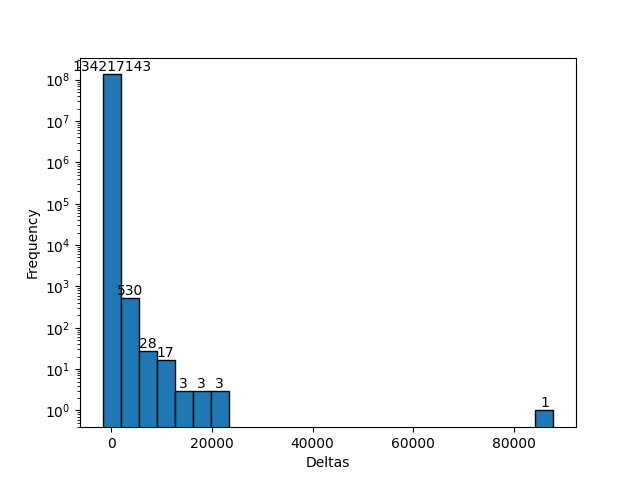
\includegraphics[width=\textwidth]{./plots_jitter/jitter_baseline/output_size_1_rank_0_25.png}
  \caption{baseline single thread\\$t=2.421950996$}
\end{subfigure}

\begin{subfigure}{.42\textwidth}
  \centering
  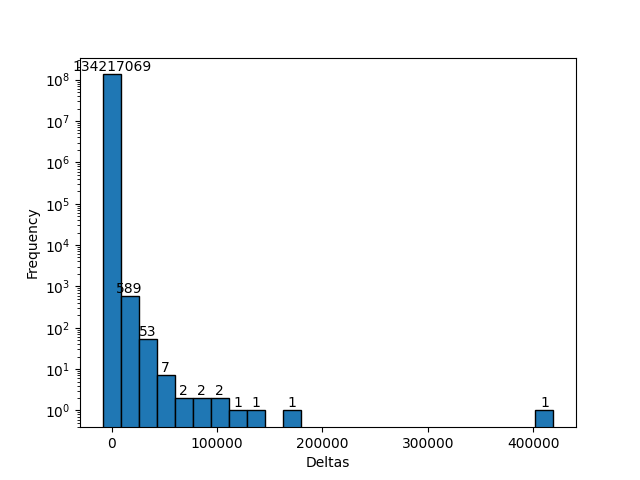
\includegraphics[width=\textwidth]{./plots_jitter/jitter/output_size_8_rank_0_25.png}
  \caption{jitter 8 MPI processes (rank 0)\\$t=5.836635677$}
\end{subfigure}%
\begin{subfigure}{.42\textwidth}
  \centering
  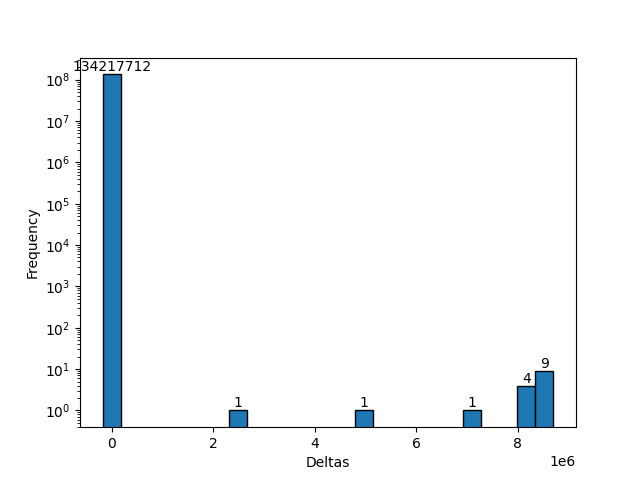
\includegraphics[width=\textwidth]{./plots_jitter/jitter_baseline/output_size_8_rank_0_25.png}
  \caption{baseline 8 MPI processes (rank 0)\\$t=5.968865865$}
\end{subfigure}

\begin{subfigure}{.42\textwidth}
  \centering
  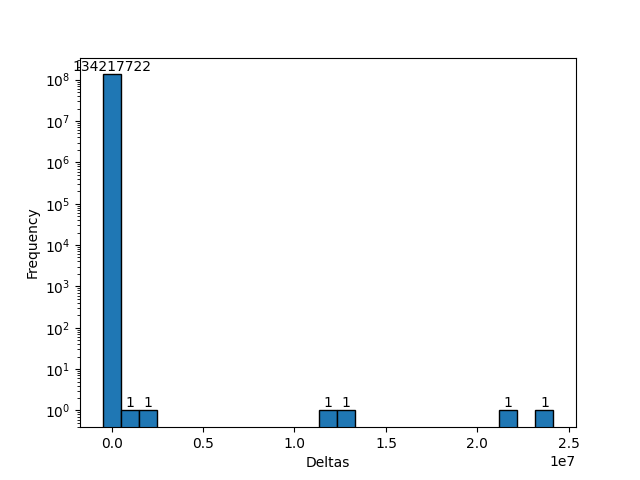
\includegraphics[width=\textwidth]{./plots_jitter/jitter/output_size_8_rank_1_25.png}
  \caption{jitter 8 MPI processes (rank 1)\\$t=5.914636448$}
\end{subfigure}%
\begin{subfigure}{.42\textwidth}
  \centering
  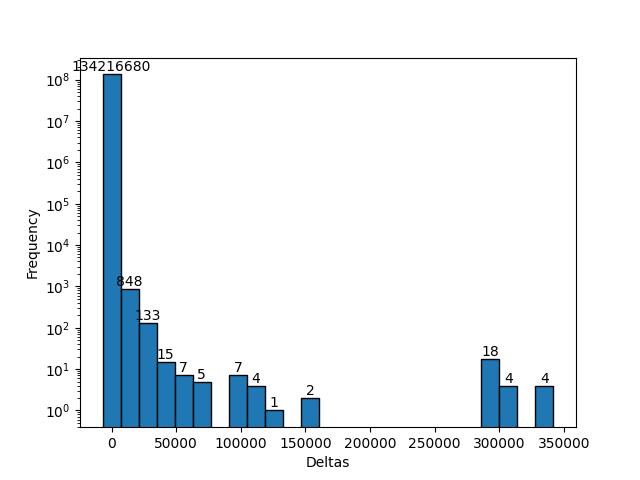
\includegraphics[width=\textwidth]{./plots_jitter/jitter_baseline/output_size_8_rank_1_25.png}
  \caption{baseline 8 MPI processes (rank 1)\\$t=5.864066244$}
\end{subfigure}
\caption{The results for single nodes, plotted onto a 25 bin, linearly sized histogram.}
\end{figure}
Due to the enormous size of the data set, a more sophisticated analysis was not possible; an in-depth reasoning is provided in the Discussion below. But it can be seen that, while a clear trend of a longer tail can be recognized, it can also be seen that this tail is very thin containing only a few data points. This implies that the performance penalty is incured just a small share of the computation time.

All pre-computed histograms for all configurations and all MPI ranks\footnote{With a bucket size of 10, 25, 50, 100 as well as calculated using the Square-root choice, Sturges Formula and Rice Rule. Also with the tail 0.05\% cut off.} as well as the fully automated benchmarking workflow and a verbose description are available in the accompanying GitHub repository.

\subsection{Prometheus}
For this benchmark, the Prometheus was configured to request each node once every 10 seconds for 10 minutes, i.e. to request each node a total of 60 times. From this maximum the theoretical max of 60 times number of nodes can be calculated. All mock clients as well as prometheus ran on the same node.

\begin{figure}[H]
  \centering
  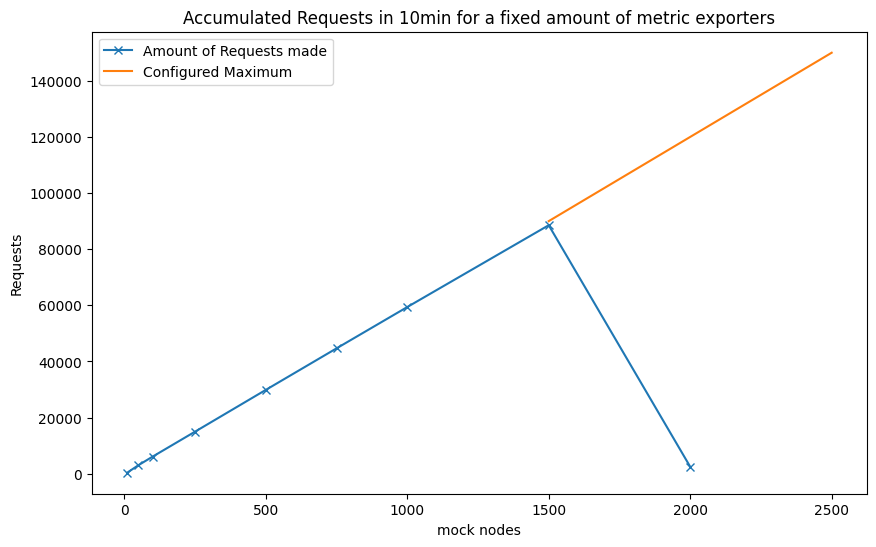
\includegraphics[width=0.7\textwidth]{./plots/prometheus_1node.png}
  \caption{Scaling up the number of mock nodes. The number of requests are the number of times Prometheus contacted one of the mock clients. All mock clients ran on a single node.}
\end{figure}

The drop off will be further analyzed in the discussion. To ensure that it is not a limitation of the Linux kernel having too many open file descriptors and running processes, the mock clients were then split onto two nodes.

\begin{figure}[H]
  \centering
  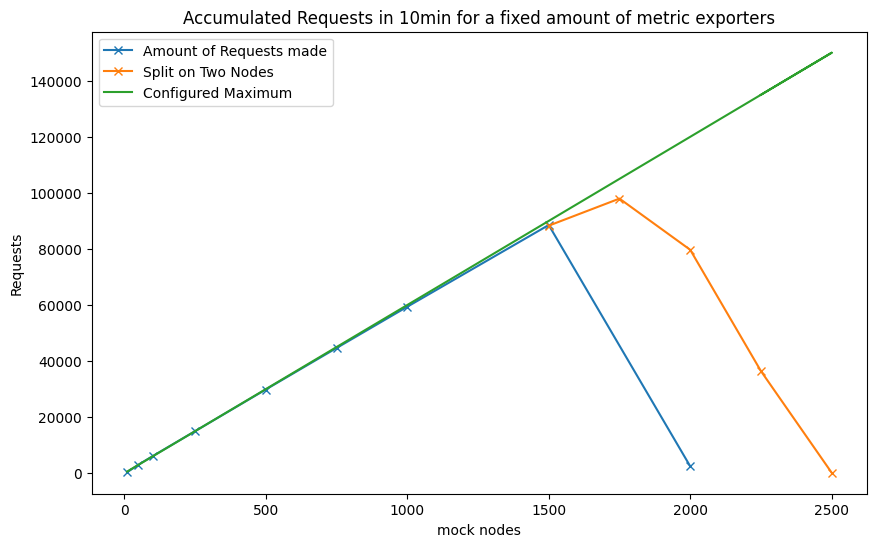
\includegraphics[width=0.7\textwidth]{./plots/prometheus_2node.png}
  \caption{Scaling up the number of mock nodes. The number of requests are the number of times Prometheus contacted one of the mock clients. The mock clients were split onto two nodes.}
\end{figure}

As one can see, using a single node, the performance drops off sharply after 1500 nodes. And even with the load split onto two nodes, it drops to nearly no requests at all using 2500 nodes. 

Excluding the dropoff itself, this performance is very bad. The data implies that, using our single node setup, monitoring more than 1500 clients would fail. Looking at the optimum case of a single node setup fetching 1500 node exporter, it approximately matches 90000 requests, which results in 150 requests per second. The metrics were of the format \texttt{keyname3: 42}. 

Assuming that each number is in the normal 32bit integer range, each metric can be rounded up to $10+\lceil\log_{10}(2^{31})\rceil = 20$ byte of data, with 50 metrics this adds up to 1kb per node. Thus a total throughput of only around 150 kb of useful data per second is achived.


\section{Discussion}
As clearly seen in the data, the Prometheus job had a scaling problem when moving from 1500 to 2000 mock node exporter. Confusingly, the problem was not CPU, Memory or I/O utilization, as all of those were not fully utilized. The data showing the utilization while benchmarking with one server running 2000 mock nodes can be found in the appendix.

The working hypothesis was that the Linux kernel had problems with that many mock processors; either handling all the open file descriptors or just scheduling the sheer amount of processes. To validate that hypothesis, the two \ac{HPC} node benchmarks were done. While the benchmark show that it scales further, it does not show that the problem was with either the amount of processes or the amount of file descriptors. When splitting the mock load generator onto two nodes, the expected result would be around twice the amount of nodes until it stops serving all collectors, which is definitely not the case\footnote{Not exactly twice the amount, because one of the nodes still ran Prometheus. Although this should not be a problem since, as already mentioned, the node was idling on all ressource dimensions.}.\\

Furthermore, one should note that the mocked \texttt{node\_exporter} used pseudorandomness\footnote{Using the warmed-up mersenne twister method mentioned in the methodology.} for the fake metric generation. While this is less realistic than using more sophisticated data generation methods such as perlin noise, it incurs significantly less overhead per fake node. Other benchmarks such as the previously mentioned \ac{TSBS} used pregenerated mock data. This would also not be possible as it would result into a very heavy I/O load on the central storage cluster, resulting in strongly reduced I/O speed for all Prometheus operations.\\

Lastly, the jitter benchmark was very difficult to analyze. Due to the inherent design on recording as many data points as possible, it resulted in over 130 million data points, sometimes recording less than 3 seconds of time. It was not possible to downsample the data since the thin long tails were explicitly of interest. The data set was too large to use kernel density estimations to create a probability density function. Furthermore, due to the sheer differences in tail latencies, layering the measurements and its baseline on the same histogram was not possible, as it was not possible to find a bin selection that properly presented both.

It was not possible to properly analyze the tail, because it was very hard to isolate. While for example with the 1 thread benchmark the tails measurements went up to the 1e6 nanoseconds range, the $p_{99.9}$ was only $786$ns. The thinness and length of the tail latencies, its range difference between the benchmarks combined with the sheer data set size made any sophisticated analysis impossible within the scope of this report. In fact, this analysis was only possible because the plots could be computed on a \ac{HPC} node; On the laptop the benchmarks were made of the process was killed, most likely due to an Python-internal out of heap memory error.

\section{Conclusion}
For this report, four methods of benchmarking the Prometheus monitoring architecture were designed and implemented, measuring both the performance of as well as performance penalty incurred by the \texttt{node\_exporter} metric collector as well as the performance and scalability of Prometheus.

The results show that, although the collector did not handle the stress test load well, its throughput and overall performance is cufficient and the collection time acceptable, even using only a single process for execution. Prometheus itself did not scale well beyond a certain amount of nodes, failing with 2000 collectors when all run on one not fully utilized \ac{HPC} node. Thus, a non clustered Prometheus solution would not be able to serve the combined load of both the SCC and Emmy cluster as Prometheus performance degrades too much immensely after a certain amount of nodes.

\subsection{Future Work}
While a simple Prometheus showed to not scale properly enough, clustered Prometheus-based solutions such as Cortex\footnote{\url{https://cortexmetrics.io/}} or Thanos\footnote{\url{https://thanos.io/}} could provide a solution able to monitor multiple \ac{HPC} clusters\footnote{The collector itself had sufficient performance.}. Possible future work includes evaluating and comparing both of these clusters.

Furthermore, in order to have a definite conclusion on the full performance penalty created by \texttt{node\_exporter}, a more sophisticated analysis has to be done. This could include identifying the tail through clustering techniques, manually cutting of the few very extreme data points for more insightful plotting or otherwise computing a cutoff for the data points.

Lastly, the Prometheus benchmark could be set up in a way that Prometheus itself is deployed isolated on a single node while all mocked collectors are distributed on different nodes. This would create a more realistic scenario with higher round trip times between all nodes.
